\documentclass[tikz,border=10pt]{standalone}
\usetikzlibrary{calc}
\begin{document}
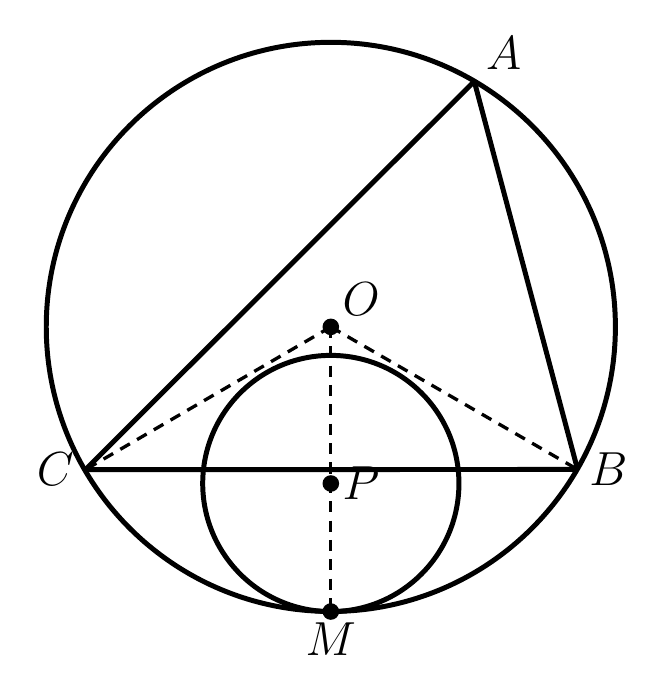
\begin{tikzpicture}[line width=1.8pt, line join=round]
  % Scale: 1 px = 0.022989 cm; origin at O (pixel 202.3,199.0), y flipped
  \coordinate (O) at (0,0);
  \coordinate (P) at (0,-1.989);      % small circle centre (CV)
  \coordinate (M) at (0,-3.615);      % tangency point, bottom of small circle
  \coordinate (A) at (1.822,3.119);
  \coordinate (B) at (3.134,-1.811);
  \coordinate (C) at (-3.115,-1.812);

  % Circles
  \draw (O) circle (3.614);           % big circle
  \draw (P) circle (1.627);           % small circle

  % Solid triangle sides and horizontal chord
  \draw (A) -- (C);
  \draw (A) -- (B);
  \draw (C) -- (B);

  % Construction lines: heavier dashes (1.2pt), longer dash pattern
  \draw[line width=1.2pt, dash pattern=on 4pt off 3pt] (O) -- (C);
  \draw[line width=1.2pt, dash pattern=on 4pt off 3pt] (O) -- (B);
  \draw[line width=1.2pt, dash pattern=on 4pt off 3pt] (O) -- (M);

  % Points: enlarged filled dots (radius about 3pt)
  \fill (O) circle (3pt);
  \fill (P) circle (3pt);
  \fill (M) circle (3pt);

  % Labels
  \node[font=\fontsize{16.5}{19.8}\selectfont, above right] at (A) {$A$};
  \node[font=\fontsize{16.5}{19.8}\selectfont, above right] at (O) {$O$};
  \node[font=\fontsize{16.5}{19.8}\selectfont, left] at (C) {$C$};
  \node[font=\fontsize{16.5}{19.8}\selectfont, right] at (B) {$B$};
  \node[font=\fontsize{16.5}{19.8}\selectfont, right] at (P) {$P$};
  \node[font=\fontsize{16.5}{19.8}\selectfont, below] at (M) {$M$};
\end{tikzpicture}
\end{document}